\chapter{Visualization System}
In this chapter the system architecture and corresponding components will be introduced. This chapter emphasizes on depicting the whole picture of the solution, some specific technical detail will be represented in the later chapters.

\section{System architecture}

The visualization system is to display the COMSOL's plots in the web application. To accomplish the goal, the system architecture in fig. 1 is needed.

\begin{figure}[htb]
  \centering
  \includegraphics[width=.9\textwidth]{Assets/System_architecture}
  \caption{System architecture}
\end{figure}

To render the graphics in the web client, the source data need to be extracted and converted at first. COMSOL provides the COMSOL Java API(CJAPI) to handle with its mph file. To use the CJAPI, a Java application is needed. The Java application can access into the model object and extract the meta information and binary data of plots, then export the required data separately into JavaScript Object Notation(JSON) file and binary file. Via a Secure File Transfer Protocol(SFTP), the files are committed to the web server. As the back-end, web server provides the web application and all the necessary data for visualization. The web server is built by Node.js, which is based on Google's JavaScript run-time environment. Its event-driven architecture and asynchronous I/O capability bring about good performance while loading large volume data. To meet the needs of dynamic reload of plots' data, a bidirectional connection protocol WebSocket is used between web server and web client. Since that web client runs on various browsers and devices, the compatibility must be considered. The web client is responsive design for both mobile and desktop devices and a universal UI(User Interface) is built with HTML5 standard and display the visualization results. Besides, user interaction is also supported for post-processing with the rendered graphics. For more user experience, the stereo display can be enable with 3D screen, and Virtual Reality(VR) experience could also be provided with VR headsets.

\section{Data processing}

 The core task of a visualization system is about data processing, the graphics data needs to be extracted from original file and converted correctly for the usage of web client before presenting. All results or plot data can be retrieved directly through the COMSOL API\cite{COMSOL Programming reference manual}. In the figure 2, the data convert process is shown.

 \begin{figure}[htb]
  \centering
  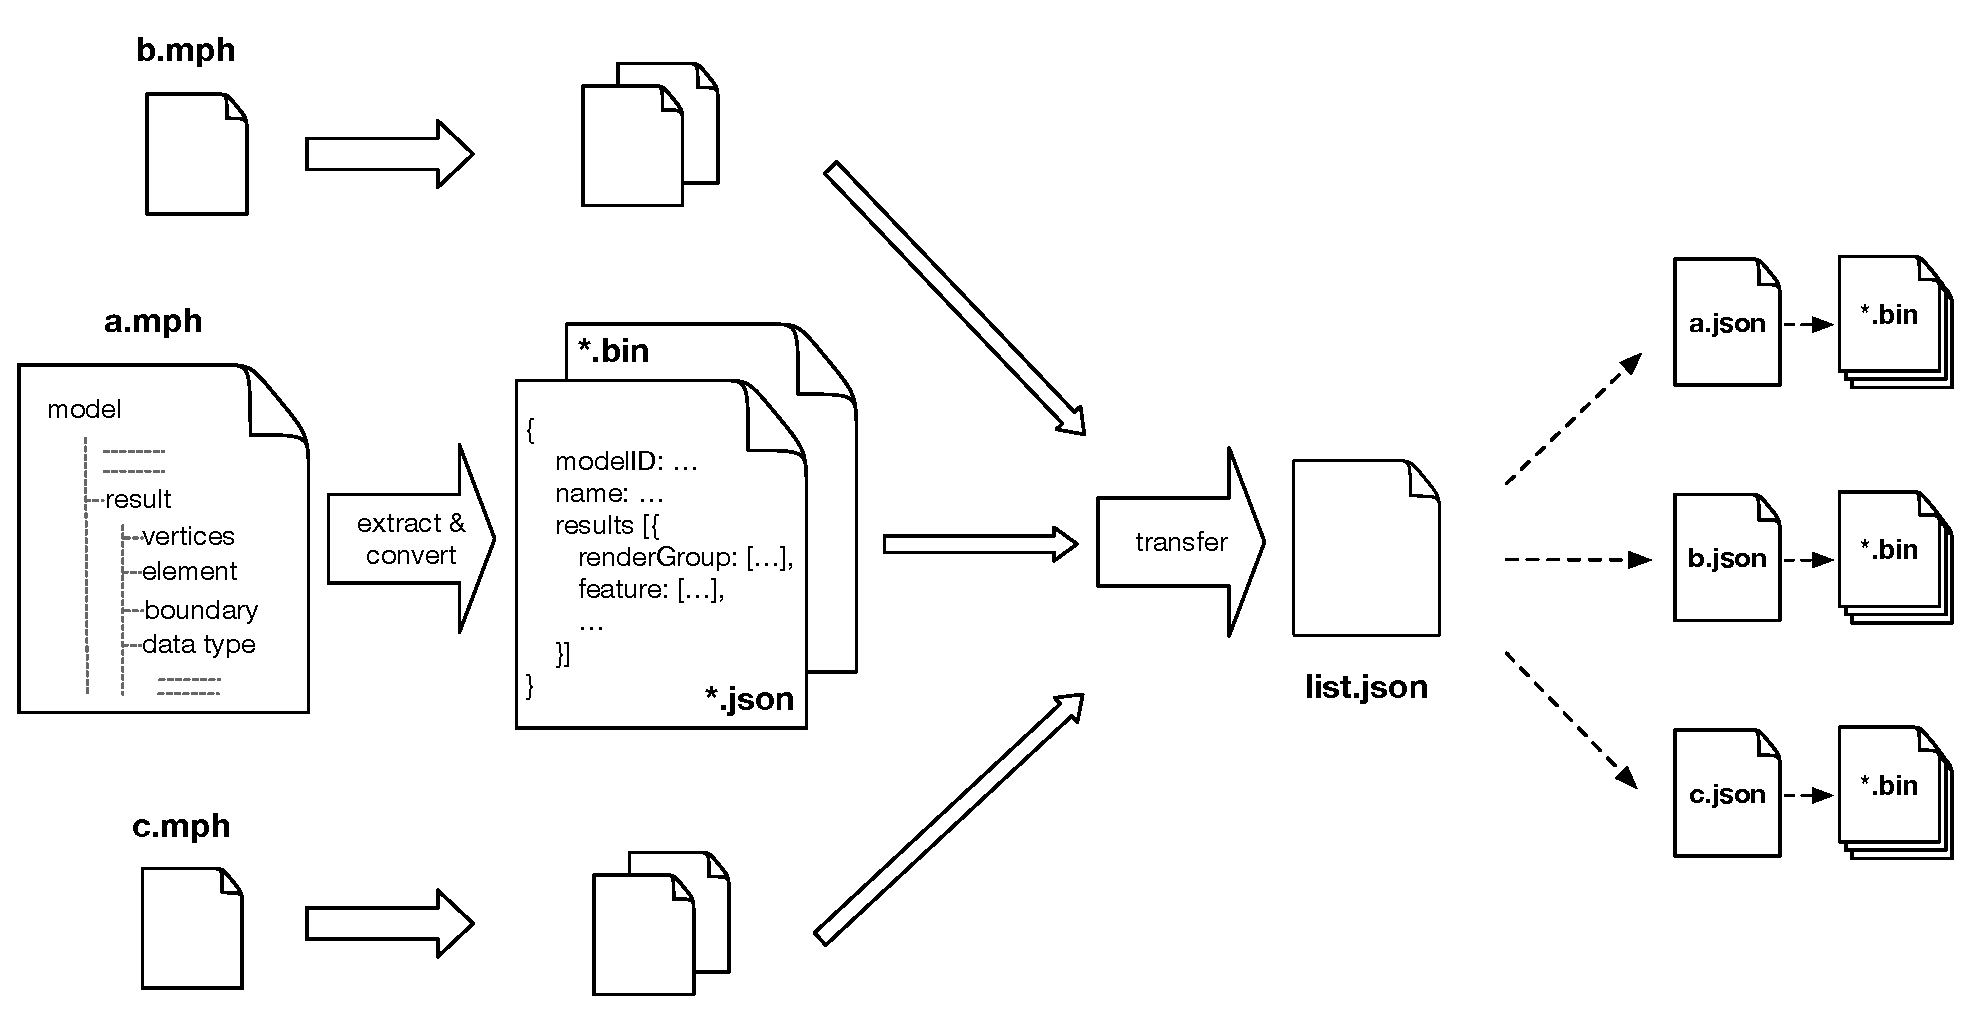
\includegraphics[width=.9\textwidth]{Assets/Data_convert}
  \caption{Data flow}
\end{figure}

The model is organized in tree structure and CJAPI provides direct access through the model object.

The detailed model structure are detail in COMSOL Multiphysics Programming Reference Manual\cite{} 